\chapter{Data Preparation}

\vspace*{1cm}

Data preparation is an important step in this project because the quality and
format of the dataset directly affect the fine-tuning process. The model used in
this work expects text inputs and text outputs, so the original dataset must be
converted into a clear instruction-tuning format before training.

\section{Dataset Description}

The dataset used in this project is \texttt{yahma/alpaca-cleaned}. It is a cleaned
instruction-following dataset based on the Alpaca format. Each example generally
contains an instruction, an optional input, and an output. This structure makes it
suitable for adapting a language model to follow user instructions.

\vspace*{0.5cm}

The dataset is downloaded using the Hugging Face \texttt{datasets} library. The
configured split used in the project is the training split of the dataset. From
this split, smaller subsets are created in order to keep the experiment light and
adapted to the available computational resources.

\begin{figure}[H]
    \centering
    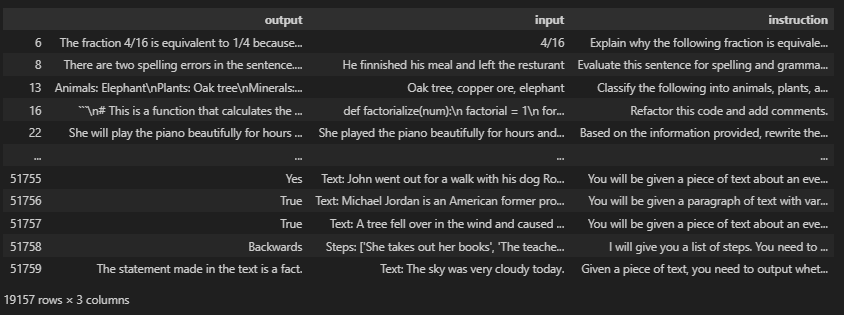
\includegraphics[width=0.95\textwidth]{chapters/images/dataset_examples.png}
    \caption{Examples extracted from the original instruction-following dataset.}
    \label{fig:dataset_examples}
\end{figure}

\section{Configuration}

The data preparation parameters are stored in the project configuration file
\texttt{config.yaml}. This file defines the dataset name, the split to use, the
output directory, the random seed, and the number of examples for each subset.

\vspace*{0.5cm}

The current configuration uses the following values:

\begin{table}[H]
    \centering
    \begin{tabular}{ll}
        \toprule
        \textbf{Parameter} & \textbf{Value} \\
        \midrule
        Dataset name & \texttt{yahma/alpaca-cleaned} \\
        Dataset split & \texttt{train} \\
        Training size & 2000 examples \\
        Validation size & 500 examples \\
        Test size & 500 examples \\
        Random seed & 42 \\
        Output directory & \texttt{data/processed} \\
        \bottomrule
    \end{tabular}
    \caption{Main data preparation configuration.}
    \label{tab:data_config}
\end{table}

\begin{figure}[H]
    \centering
    \includegraphics[width=0.95\textwidth]{chapters/images/yaml-config.png}
    \caption{yaml configuration for data preparation.}
    \label{fig:yaml_config}
\end{figure}

\section{Processing Steps}

The data preparation script is implemented in \texttt{src/prepare\_data.py}. Its
role is to transform the original dataset into files that can be used directly by
the fine-tuning pipeline.

\vspace*{0.5cm}

The processing pipeline follows these steps:

\begin{enumerate}
    \item Load the configuration from \texttt{config.yaml}.
    \item Download the dataset \texttt{yahma/alpaca-cleaned}.
    \item Shuffle the dataset using the configured seed.
    \item Select the training, validation, and test subsets.
    \item Clean missing or empty text fields.
    \item Convert each example into an instruction-tuning format.
    \item Save the processed files in \texttt{CSV} and \texttt{JSONL} formats.
    \item Compute and save dataset statistics.
\end{enumerate}

\section{Instruction-Tuning Format}

The original dataset contains three main fields: \texttt{instruction},
\texttt{input}, and \texttt{output}. During preprocessing, these fields are
converted into two columns used by the model:

\begin{itemize}
    \item \texttt{source\_text}: the input prompt given to the model.
    \item \texttt{target\_text}: the expected answer generated by the model.
\end{itemize}

\vspace*{0.5cm}

If the original example contains an input, the source text is formatted as:

\begin{lstlisting}[style=jsonStyle]
Instruction: <instruction>
Input: <input>
Answer:
\end{lstlisting}

If the original example does not contain an input, the source text is formatted
as:

\begin{lstlisting}[style=jsonStyle]
Instruction: <instruction>
Answer:
\end{lstlisting}

The target text corresponds to the original output:

\begin{lstlisting}[style=jsonStyle]
<output>
\end{lstlisting}

\section{Generated Files}

After preprocessing, the processed dataset is saved in the
\texttt{data/processed/} directory. The project stores each subset in two
formats. The \texttt{CSV} format is useful for quick inspection and analysis,
while the \texttt{JSONL} format is suitable for machine learning pipelines.

\vspace*{0.5cm}

The generated files are:

\begin{itemize}
    \item \texttt{train.csv}
    \item \texttt{validation.csv}
    \item \texttt{test.csv}
    \item \texttt{train.jsonl}
    \item \texttt{validation.jsonl}
    \item \texttt{test.jsonl}
    \item \texttt{dataset\_stats.json}
\end{itemize}

\section{Dataset Statistics}

The preprocessing script also computes useful statistics about the processed
dataset. These statistics help verify the size of each subset and the average
length of the generated prompts and answers.

\begin{figure}[H]
    \centering
    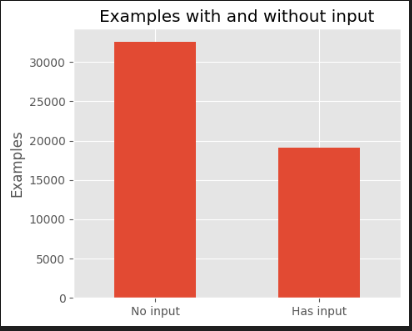
\includegraphics[width=0.65\textwidth]{chapters/images/input_distribution.png}
    \caption{Distribution of examples with and without input in the dataset.}
    \label{fig:input_distribution}
\end{figure}

\vspace*{0.5cm}

\begin{table}[H]
    \centering
    \begin{tabular}{lr}
        \toprule
        \textbf{Statistic} & \textbf{Value} \\
        \midrule
        Original examples & 51760 \\
        Training examples & 2000 \\
        Validation examples & 500 \\
        Test examples & 500 \\
        Average source length & 17.14 words \\
        Average target length & 109.21 words \\
        Maximum source length & 279 words \\
        Maximum target length & 450 words \\
        \bottomrule
    \end{tabular}
    \caption{Statistics of the processed dataset.}
    \label{tab:data_stats}
\end{table}

\section{Conclusion}

The data preparation step produces a clean and structured dataset for
instruction-tuning \texttt{google/flan-t5-small}. By converting the original
examples into \texttt{source\_text} and \texttt{target\_text}, the project creates
a direct bridge between the dataset and the fine-tuning pipeline. This prepared
data is then used in the next stage to train and compare the selected
optimization algorithms.
